\section[Le architetture]{Le architetture}
\label{sec:architectures}
\sectionframe{images/covers/cover_architecture.jpeg}{Le Architetture}


\subsection[La macchina di Turing]{La macchina di Turing}
\begin{frame}
	\frametitle{La macchina di Turing}
	 
	\begin{block}{Il computer}
		Il computer è un dispositivo fisico che implementa il funzionamento di una macchina di Turing.
	\end{block}
	\begin{block}{La Macchina di Turing}
		La Macchina di Turing è una macchina ideale che manipola i dati contenuti su un nastro di lunghezza potenzialmente infinita, secondo un insieme prefissato di regole ben definite.\\
		In altre parole, si tratta di un modello astratto che definisce una macchina in grado di eseguire algoritmi e dotata di un nastro potenzialmente infinito su cui può leggere e/o scrivere dei simboli.
	\end{block}
\end{frame}



\begin{frame}
	\frametitle{La macchina di Turing}
	
	\begin{block}{Una simulazione della Macchina di Turing}
		\begin{figure}[!htbp]
			\centering 
			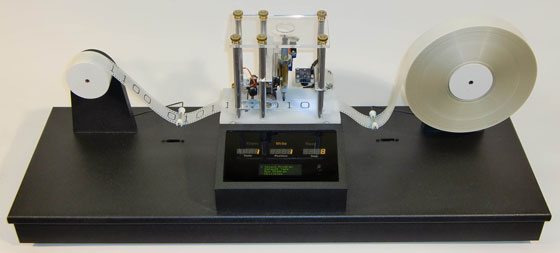
\includegraphics[width=0.9\linewidth]{images/2_le_architetture/turing_machine.jpg}
			\caption{Foto da \href{https://aturingmachine.com/}{aturingmachine.com}, clicca \underline{\href{https://www.youtube.com/watch?v=E3keLeMwfHY}{qui}} per vedere il video.}
			\label{fig:architectures_turingmachine}
		\end{figure}
	\end{block}
\end{frame}


\subsection[Il computer]{Il computer}
\begin{frame}
	\frametitle{Il computer}
	
	\begin{block}{Il computer}
		Un computer esegue programmi (come la macchina di Turing).\\
		Esistono due categorie di computer:
		\begin{columns}			
			\column{0.3\linewidth}
			\begin{figure}[!htbp]
				\centering 
				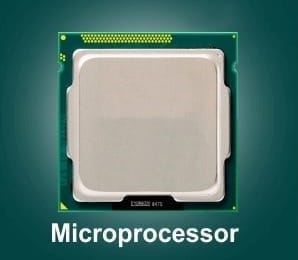
\includegraphics[width=0.7\linewidth]{images/2_le_architetture/microprocessor.jpeg}
				%\caption{}
			\end{figure}
			
			\column{0.5\linewidth}
			$\bullet$ \textbf{general purpose}:\\riprogrammabili dall'utente ($\mu$processors, utilizzati ad esempio nei \textit{personal computer}).
			
			\column{0.2\linewidth}
			\begin{figure}[!htbp]
				\centering
				\advance\leftskip-0.5cm
				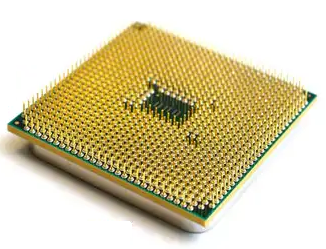
\includegraphics[width=1.0\linewidth]{images/2_le_architetture/microprocessor.png}
				%\caption{}
			\end{figure}
			
		\end{columns}
		 
		\begin{columns}						
			\column{0.3\linewidth}
			\begin{figure}[!htbp]
				\centering 
				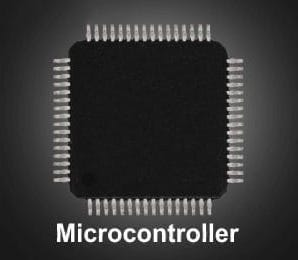
\includegraphics[width=0.7\linewidth]{images/2_le_architetture/microcontroller.jpeg}
				%\caption{}
			\end{figure}
			
			\column{0.5\linewidth}
			$\bullet$ \textbf{special purpose}:\\dedicati ad una sola applicazione specifica  ($\mu$controllers, utilizzati ad esempio negli \textit{elettrodomestici}).
			
			\column{0.2\linewidth}
			\begin{figure}[!htbp]
				\centering
				\advance\leftskip-0.5cm
				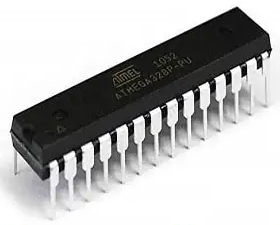
\includegraphics[width=1.0\linewidth]{images/2_le_architetture/microcontroller.png}
				%\caption{}
			\end{figure}
			
		\end{columns}
		
	\end{block}
	
	
\end{frame}



\subsection[I transistor]{I transistor}
\begin{frame}
	\frametitle{I transistor}
	
	\begin{columns}			
		\column{0.6\linewidth}
		\begin{block}{I microprocessori e i microcontrollori}
			I microprocessori e i microcontrollori sono componenti chiave dei computer e dei dispositivi elettronici in quanto ne costituiscono il "cervello".\\~\\
			Uno dei componenti elettronici più importanti all'interno di questi sono i \textbf{transistor}, utilizzati al loro interno per:
			\begin{itemize}
				\item creare \textbf{circuiti logici}, utilizzati per eseguire calcoli di logica e aritmetica e prendere decisioni,
				\item \textbf{memorizzare informazioni} al loro interno
			\end{itemize} 
		\end{block}
		
		\column{0.4\linewidth}
		\begin{figure}[!htbp]
			\centering 
			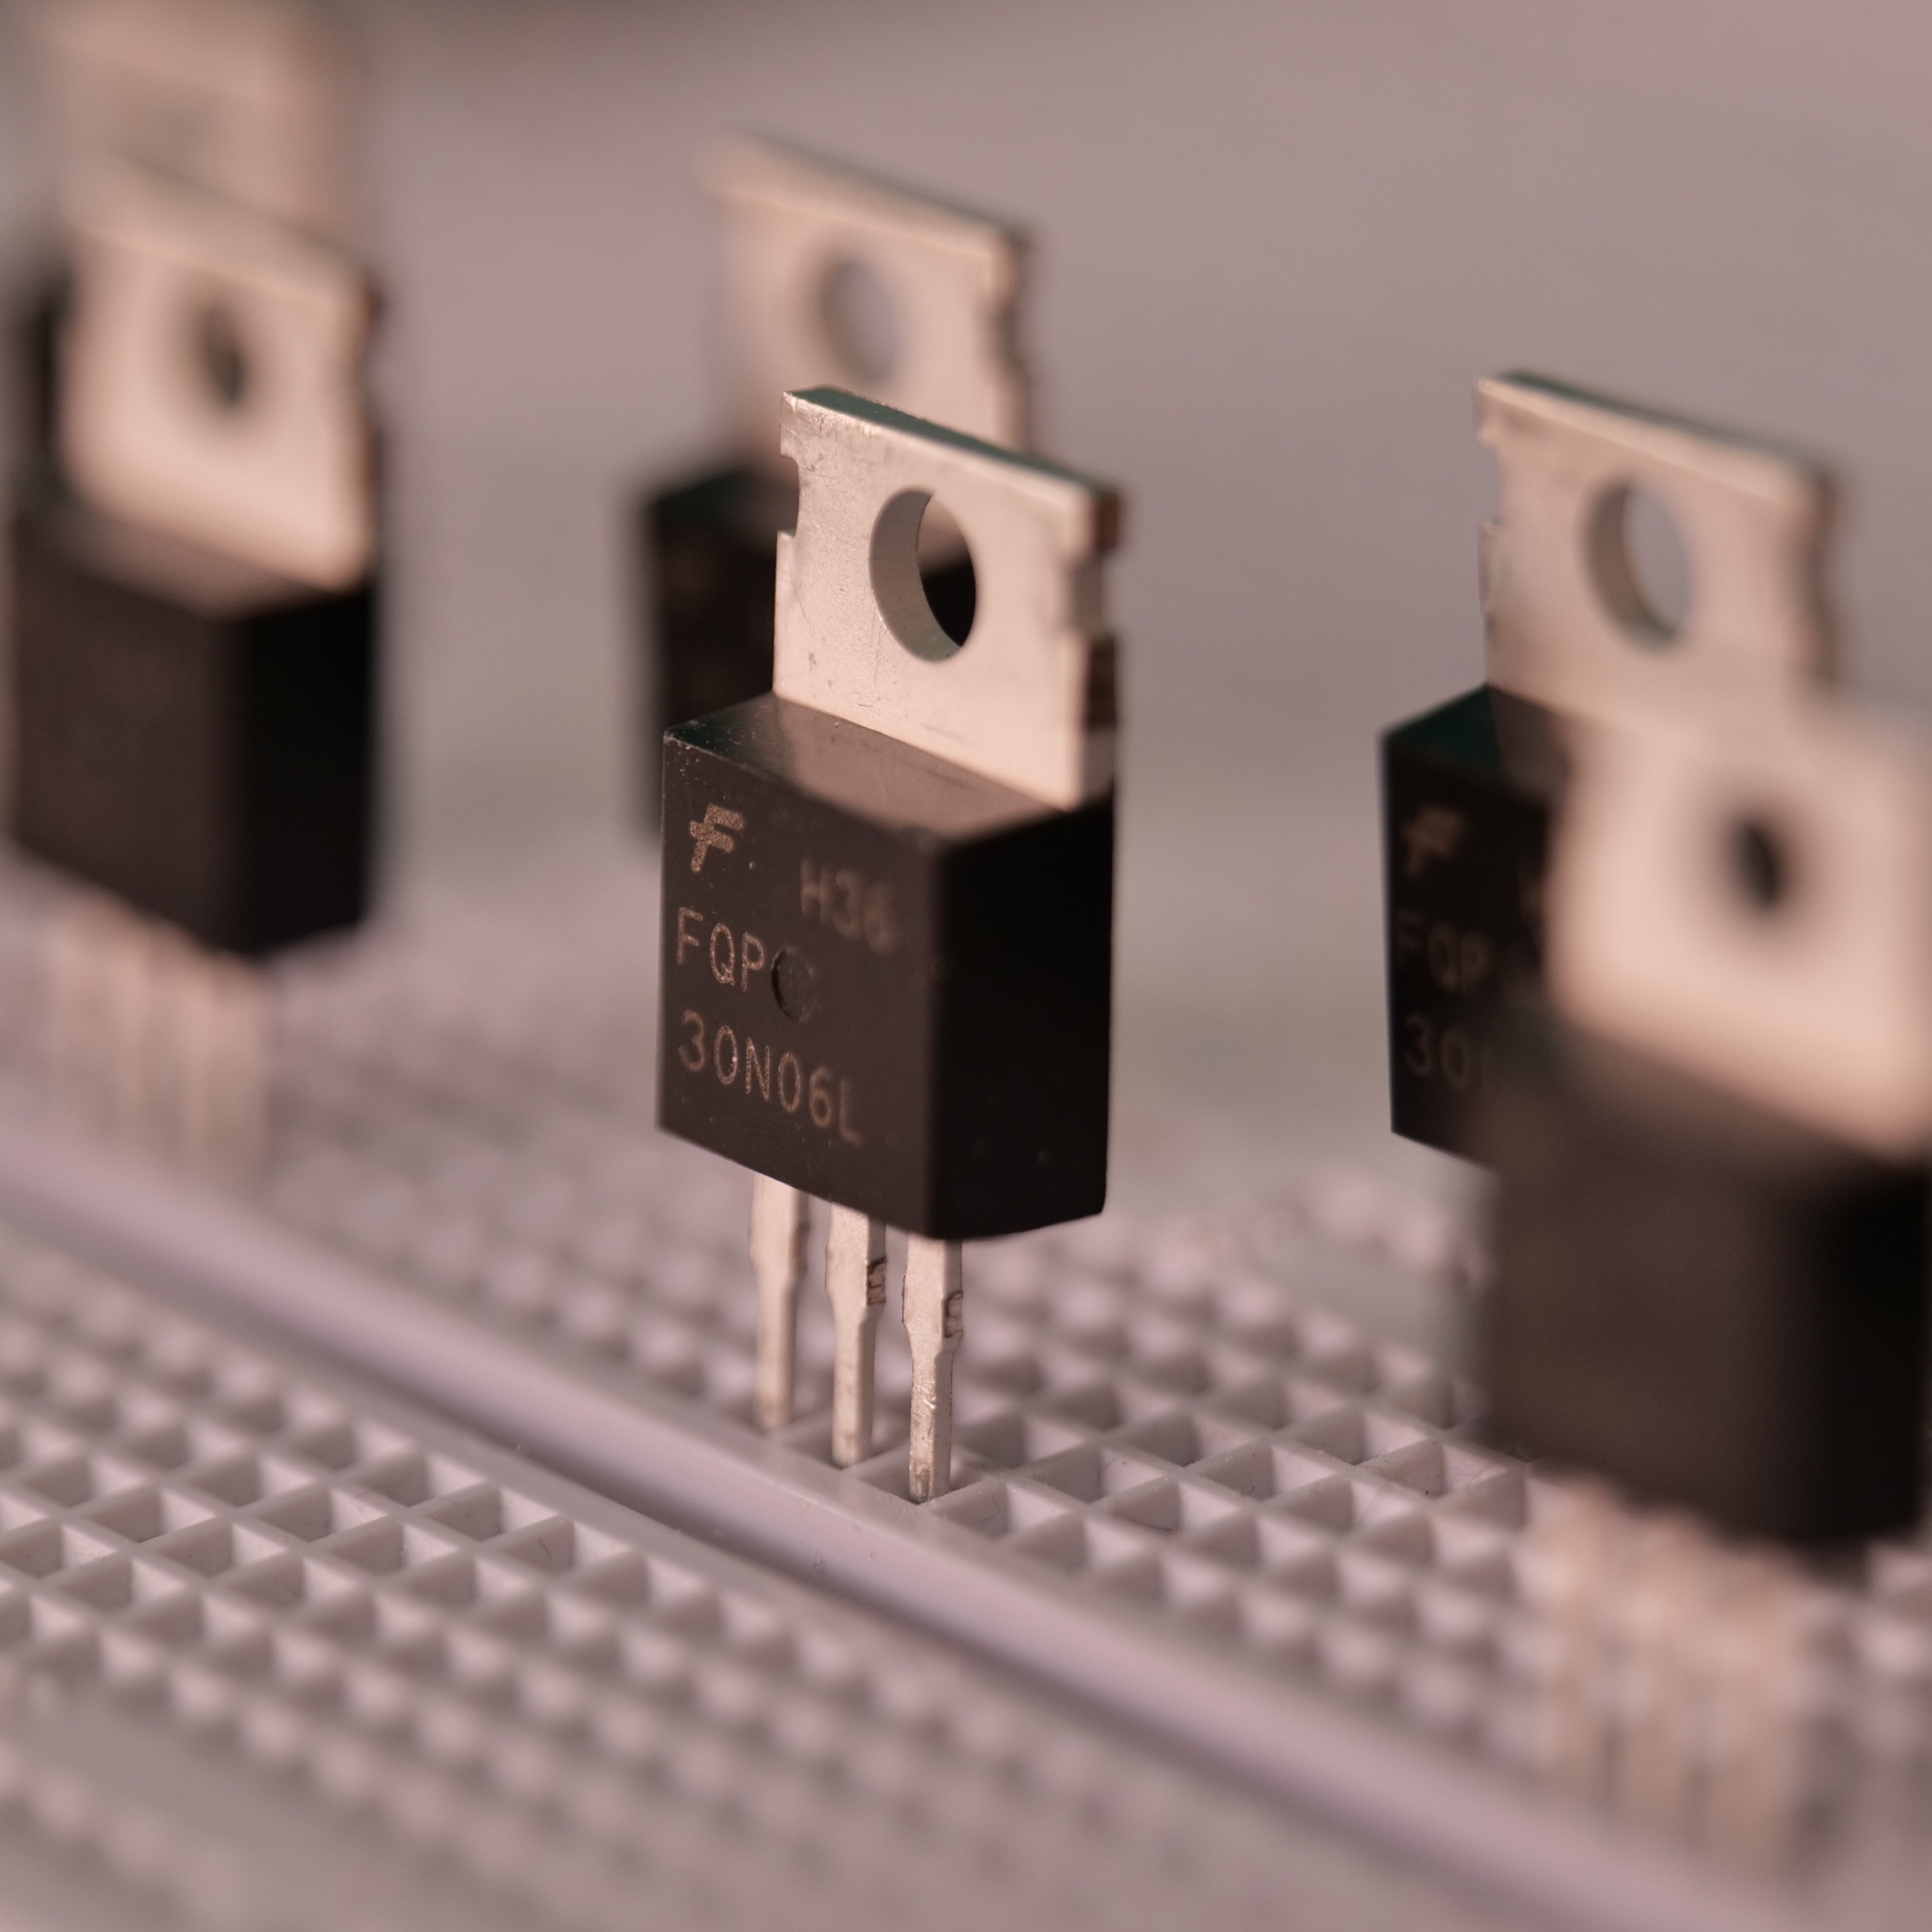
\includegraphics[width=0.95\linewidth]{images/2_le_architetture/transistor.jpg}
			\caption{Transistors}
			\label{fig:architectures_transistors}
		\end{figure}		
	\end{columns}
	
\end{frame}




\begin{frame}
	\frametitle{I Transistor}
	
	\begin{columns}			
		\column{0.6\linewidth}
		\begin{block}{I Transistor}
			I transistor sono componenti elettronici utilizzati in molti circuiti elettronici in quanto permettono di \textbf{amplificare} o \textbf{interrompere} un \textbf{segnale elettrico}.
		\end{block}
		
		\begin{block}{16 Dic 1947, Bardeen, Brattain e Shockley riuscirono a creare il primo transistor}
			all'interno degli \textbf{AT\&T Bell Laboratories} (un centro di ricerca e sviluppo, attualmente di proprietà di Nokia) da allora sono diventati un componente chiave dell'elettronica.
		\end{block}
		
		\column{0.4\linewidth}
		\begin{figure}[!htbp]
			\centering 
			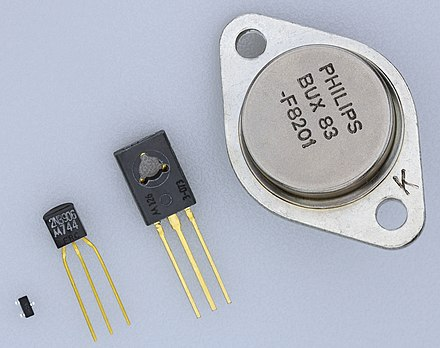
\includegraphics[width=0.95\linewidth]{images/2_le_architetture/transistors.jpg}
			\caption{Confronto tra diversi transistor BJT, da sinistra a destra: SOT-23, TO-92, TO-126, TO-3}
		\end{figure}		
	\end{columns}
	
\end{frame}



\begin{frame}
	\frametitle{I Transistor}
	
	\begin{columns}			
		\column{0.6\linewidth}
		\begin{block}{Il Nobel}
			Il transistor doveva inizialmente servire a \textbf{migliorare le comunicazioni} tra il continente americano e quello europeo oggi lo troviamo impiegato nei campi più disparati (informatica, telefonia, smart-car, radio, ...).\\~\\
			Nel \textbf{1956} i tre scienziati statunitensi hanno ricevuto il \textbf{Premio Nobel per la Fisica} per gli studi condotti all'interno dei laboratori di ricerca e sviluppo dell'AT\&T: in appena 9 anni il transistor è diventato una delle componenti hardware più importanti e utilizzate in ambito elettronico.
		\end{block}
		
		\column{0.4\linewidth}
		\begin{figure}[!htbp]
			\centering 
			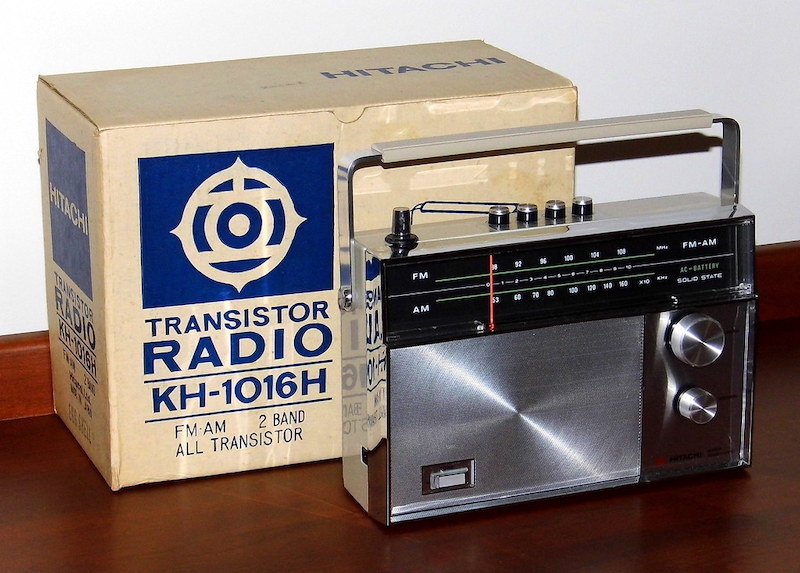
\includegraphics[width=0.95\linewidth]{images/2_le_architetture/radio_transistors.jpeg}
			\caption{I transistor sono usati nelle radio sia per amplificare il segnale radiofonico   ricevuto dall'antenna che per il circuito di sintonizzazione utilizzato per selezionare la frequenza del segnale radiofonico.}
		\end{figure}		
	\end{columns}
	
\end{frame}


\subsection[La capacità di integrazione]{La capacità di integrazione}
\begin{frame}
	\frametitle{La capacità di integrazione}
	
	\begin{block}{La capacità di integrazione}
		Si definisce \textbf{capacità di integrazione} la misura di quanti transistor sono realizzati all'interno di un unico chip integrato:
		\begin{itemize}
			\item SSI (Small Scale Integration): $\qquad\quad\,$ < 100 transistor
			\item MSI (Medium Scale Integration): $\quad\;\;\:$ < 1000 transistor
			\item LSI (Large Scale of Integration): $\quad\;\;\,\,\,$ < 10.000 transistor
			\item VLSI (Very Large Scale Integration): $\,\,$ < 100.000 transistor
			\item ULSI (Ultra Large Scale Integration): $\,$ > 100.000 transistor
		\end{itemize}
		
	\end{block}
	
\end{frame}


\subsection[La legge di Moore]{La legge di Moore}
\begin{frame}
	\frametitle{La legge di Moore}
	
	\begin{block}{$\qquad$La legge di Moore}
		\begin{quote}
			La complessità di un microcircuito, misurata ad esempio tramite il numero di transistor per chip, raddoppia ogni 18 mesi (e quadruplica quindi ogni 3 anni).
		\end{quote}		
	\end{block}
	
	\pause
	
	\begin{block}{La storia dietro l'enunciato}
		Nel 1965 \textbf{Gordon Moore} (cofondatore di Intel con Robert Noyce) ipotizzò che il numero di transistori nei microprocessori sarebbe raddoppiato ogni \textbf{12 mesi} circa. 	La legge viene riformulata alla fine degli anni ottanta ed elaborata nella sua forma definitiva, ovvero che il numero di transistori nei processori raddoppia ogni \textbf{18 mesi}.\\
		Questa legge è diventata il metro e l'obiettivo di tutte le aziende che operano nel settore come Intel e AMD.
	\end{block}
	
\end{frame}


\begin{frame}
%	\frametitle{La legge di Moore}
	
%	\begin{block}{Evoluzione del numero di transistors nei microprocessori 1971-2008}
		\begin{figure}[!htbp]
			\centering
			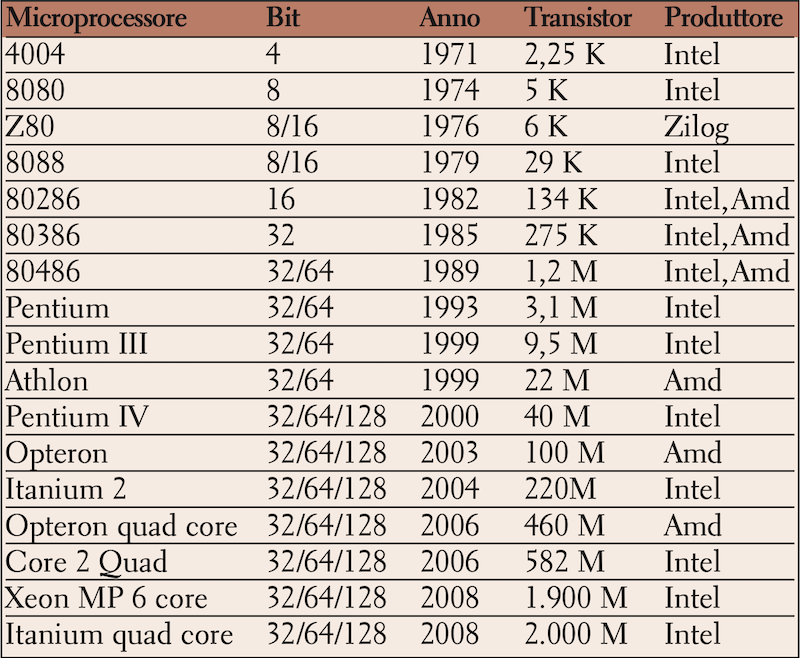
\includegraphics[width=0.7\linewidth]{images/2_le_architetture/moore.png}
			\caption{Evoluzione del numero di transistors nei microprocessori 1971-2008}
		\end{figure}
%	\end{block}

	
	
\end{frame}


\begin{frame}
%	\frametitle{La legge di Moore}
	
	\begin{figure}[!htbp]
		\centering 
		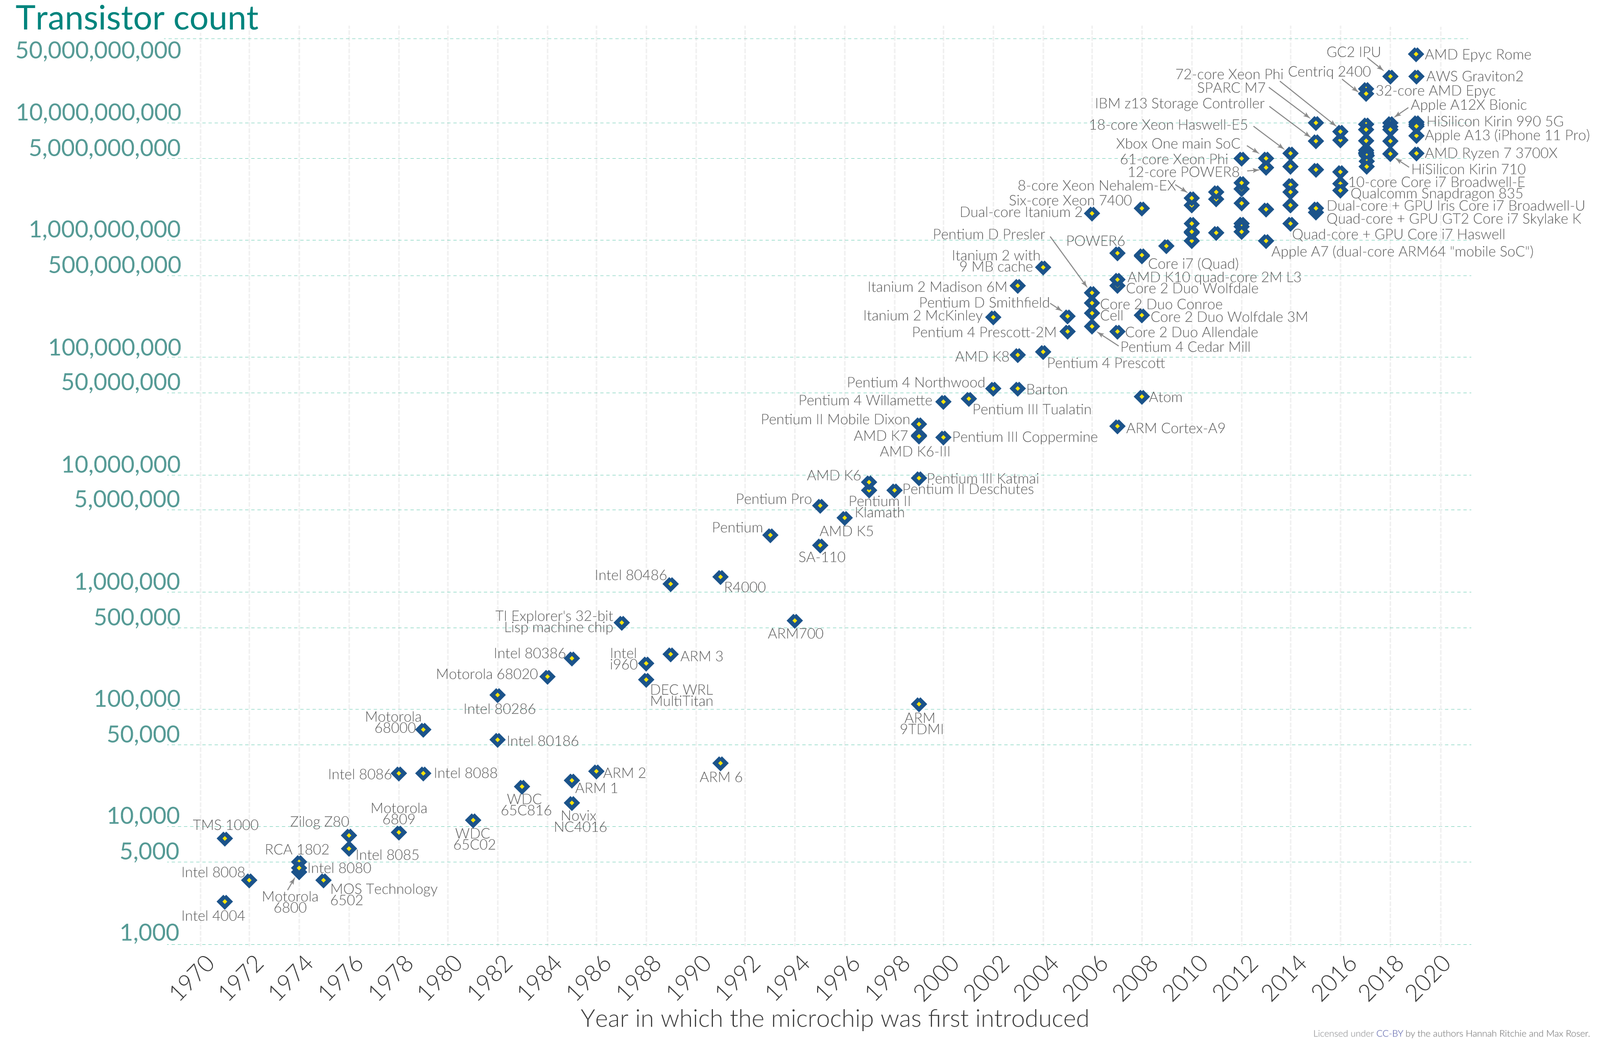
\includegraphics[width=1.02\linewidth]{images/2_le_architetture/Moore's_Law_Transistor_Count_1970-2020.png}
%		\caption{}
		\label{fig:architectures_moorelaw}	
	\end{figure}
	
\end{frame}



\subsection[Le porte logiche]{Le porte logiche}
\begin{frame}
	\frametitle{Le porte logiche}
	
	\begin{block}{Le porte logiche}
		Grazie ai transistor è possibile realizzare dei circuiti logici (vedi \hyperlink{fig:architectures_transistors}{pag. \pageref{fig:architectures_transistors}}).\\
		Le \textbf{porte logiche} sono dei circuiti elettronici elementari in grado di svolgere le operazioni logiche dell'algebra booleana basata sui valori logici:
		\begin{itemize}
			\item \textbf{TRUE} oppure \textbf{1}: passaggio di corrente (tensione alta)
			\item \textbf{FALSE} oppure \textbf{0}: non passaggio di corrente (tensione bassa)
		\end{itemize}
	\end{block}
	$\qquad\qquad\qquad\qquad\qquad\!$Le tre porte principali sono:
	
	\begin{columns}
		\column{0.33\linewidth}
		\begin{figure}[!htbp]
			\centering 
			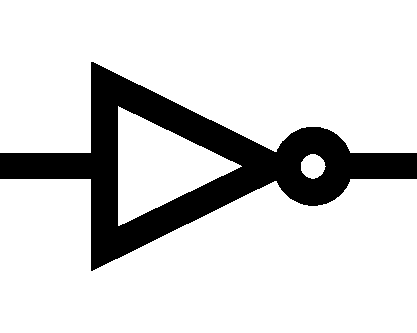
\includegraphics[width=0.5\linewidth]{images/2_le_architetture/logic_gate_not.pdf}
			\caption{Porta logica \textit{NOT}}
		\end{figure}
		
		\column{0.33\linewidth}
		\begin{figure}[!htbp]
			\centering 
			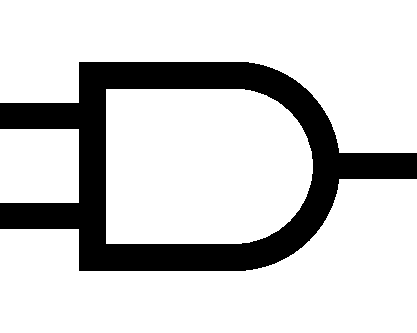
\includegraphics[width=0.5\linewidth]{images/2_le_architetture/logic_gate_and.pdf}
			\caption{Porta logica \textit{AND}}
		\end{figure} 
		
		\column{0.33\linewidth}
		\begin{figure}[!htbp] 
			\centering 
			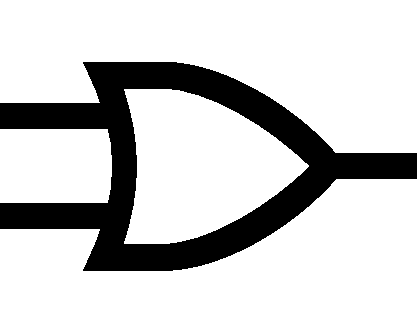
\includegraphics[width=0.5\linewidth]{images/2_le_architetture/logic_gate_or.pdf}
			\caption{Porta logica \textit{OR}}
		\end{figure}
		
	\end{columns}
	
\end{frame}


\subsubsection[La porta logica NOT]{La porta logica NOT}
\begin{frame}
	\frametitle{La porta logica NOT}
	
	
	\begin{block}{La porta logica NOT}
		è la porta logica che implementa la \textbf{negazione logica}.\\Tale dispositivo restituisce il \textbf{valore negato del livello logico} in ingresso.
	\end{block}

	\begin{columns}
		\column{0.3\linewidth}
		\begin{figure}[!htbp]
			\centering 
			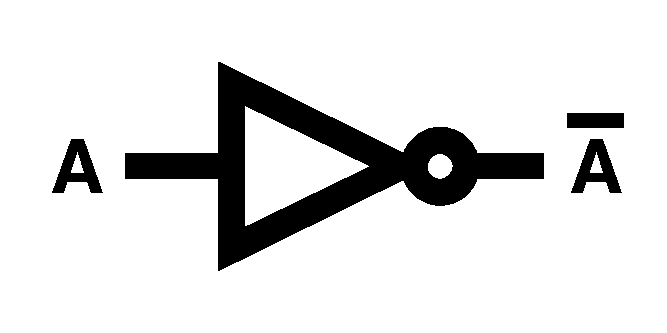
\includegraphics[width=0.9\linewidth]{images/2_le_architetture/logic_gate_not_a.pdf}
			\caption{Icona}
		\end{figure}
		
		\column{0.4\linewidth}
		\begin{table}[]
		\begin{tabular}{|
		>{\columncolor[HTML]{C0C0C0}}c |c|}
		\hline
		\cellcolor[HTML]{EFEFEF}\textbf{A} & \cellcolor[HTML]{EFEFEF}\textbf{NOT A} \\ \hline
		0                                  & 1                                      \\ \hline
		1                                  & 0                                      \\ \hline
		\end{tabular}
		\caption{Tabella di verità}
		\end{table}
		
		\column{0.3\linewidth}
		\begin{figure}[!htbp]
			\centering 
			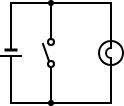
\includegraphics[width=0.85\linewidth]{images/2_le_architetture/logic_gate_circuit_not.png}
			\caption{Circuito}
		\end{figure}
		
	\end{columns}
	
\end{frame}



\subsubsection[La porta logica AND]{La porta logica AND}
\begin{frame}
	\frametitle{La porta logica AND}
	
	
	\begin{block}{La porta logica AND}
		è la porta logica che implementa la \textbf{congiunzione logica}.\\
		L'uscità è alta (a 1) solo se entrambi i valori di input A e B sono alti, in tutti gli altri casi l'uscita è bassa (a 0).\\
		In altre parole, la funzione AND corrisponde a trovare il minimo tra due cifre binarie (o a un prodotto tra due cifre binarie).
	\end{block}

	\begin{columns}
		\column{0.3\linewidth}
		\begin{figure}[!htbp]
			\centering 
			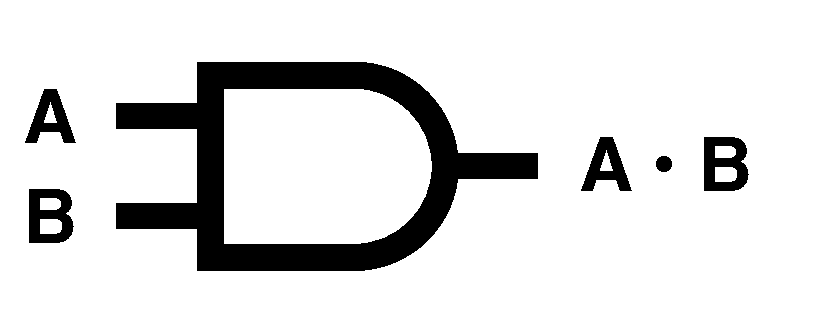
\includegraphics[width=1.0\linewidth]{images/2_le_architetture/logic_gate_and_ab.pdf}
			\caption{Icona}
		\end{figure}
		
		\column{0.4\linewidth}
		\begin{table}[]
		\begin{tabular}{|
		>{\columncolor[HTML]{C0C0C0}}c |
		>{\columncolor[HTML]{C0C0C0}}c |c|}
		\hline
		\cellcolor[HTML]{EFEFEF}\textbf{A} & \cellcolor[HTML]{EFEFEF}\textbf{B} & \cellcolor[HTML]{EFEFEF}\textbf{A $\bullet$ B} \\ \hline
		0                                  & 0                         & 0                                    \\ \hline
		0                                  & 1                         & 0                                    \\ \hline
		1                                  & 0                         & 0                                    \\ \hline
		1                                  & 1                         & 1                                    \\ \hline
		\end{tabular}
		\caption{Tabella di verità}
		\end{table}
		
		\column{0.3\linewidth}
		\begin{figure}[!htbp]
			\centering 
			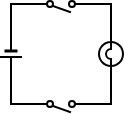
\includegraphics[width=0.85\linewidth]{images/2_le_architetture/logic_gate_circuit_and.png}
			\caption{Circuito}
		\end{figure}
		
	\end{columns}
	
\end{frame}


\subsubsection[La porta logica OR]{La porta logica OR}
\begin{frame}
	\frametitle{La porta logica OR}
	
	
	\begin{block}{La porta logica OR}
		è la porta logica digitale che implementa la \textbf{disgiunzione logica}.\\
		L'uscità è bassa (a 0) solo se entrambi i valori di input A e B sono bassi, in tutti gli altri casi l'uscita è alta (a 1).\\
		In altre parole, la funzione OR corrisponde a trovare il massimo tra due cifre binarie.
	\end{block}

	\begin{columns}
		\column{0.3\linewidth}
		\begin{figure}[!htbp]
			\centering 
			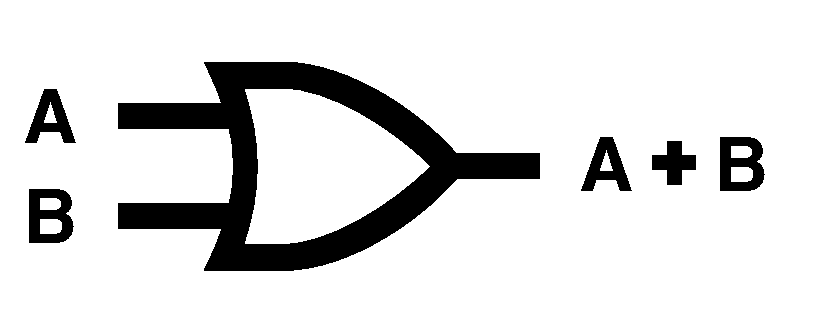
\includegraphics[width=1.0\linewidth]{images/2_le_architetture/logic_gate_or_ab.pdf}
			\caption{Icona}
		\end{figure}
		
		\column{0.4\linewidth}
		\begin{table}[]
		\begin{tabular}{|
		>{\columncolor[HTML]{C0C0C0}}c |
		>{\columncolor[HTML]{C0C0C0}}c |c|}
		\hline
		\cellcolor[HTML]{EFEFEF}\textbf{A} & \cellcolor[HTML]{EFEFEF}\textbf{B} & \cellcolor[HTML]{EFEFEF}\textbf{A $+$ B} \\ \hline
		0                                  & 0                         & 0                                    \\ \hline
		0                                  & 1                         & 1                                    \\ \hline
		1                                  & 0                         & 1                                    \\ \hline
		1                                  & 1                         & 1                                    \\ \hline
		\end{tabular}
		\caption{Tabella di verità}
		\end{table}
		
		\column{0.3\linewidth}
		\begin{figure}[!htbp]
			\centering 
			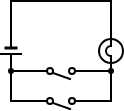
\includegraphics[width=0.85\linewidth]{images/2_le_architetture/logic_gate_circuit_or.png}
			\caption{Circuito}
		\end{figure}
		
	\end{columns}
	
\end{frame}



\subsubsection[Altre porte logiche: XOR, NAND, NOR, XNOR]{Altre porte logiche: XOR, NAND, NOR, XNOR}
\begin{frame}
	\frametitle{Altre porte logiche: XOR, NAND, NOR, XNOR}
	
	
	\begin{block}{Altre porte logiche: XOR, NAND, NOR, XNOR}
		Esistono altre porte logiche oltre a NOT, AND e OR.\\
		Tra le più importanti citiamo:
		\begin{itemize}
			\item XOR: l'OR esclusivo
			\item NAND: l'AND negato
			\item NOR: l'OR negato
			\item XNOR: lo XOR negato
		\end{itemize}
	\end{block}
	
\end{frame}


\subsubsection[Tabelle di verità: AND, OR, XOR, NAND, NOR e XNOR]{Tabelle di verità: AND, OR, XOR, NAND, NOR e XNOR}
\begin{frame}
	\frametitle{Tabelle di verità: AND, OR, XOR, NAND, NOR e XNOR}

	\begin{figure}[!htbp]
		\centering 
		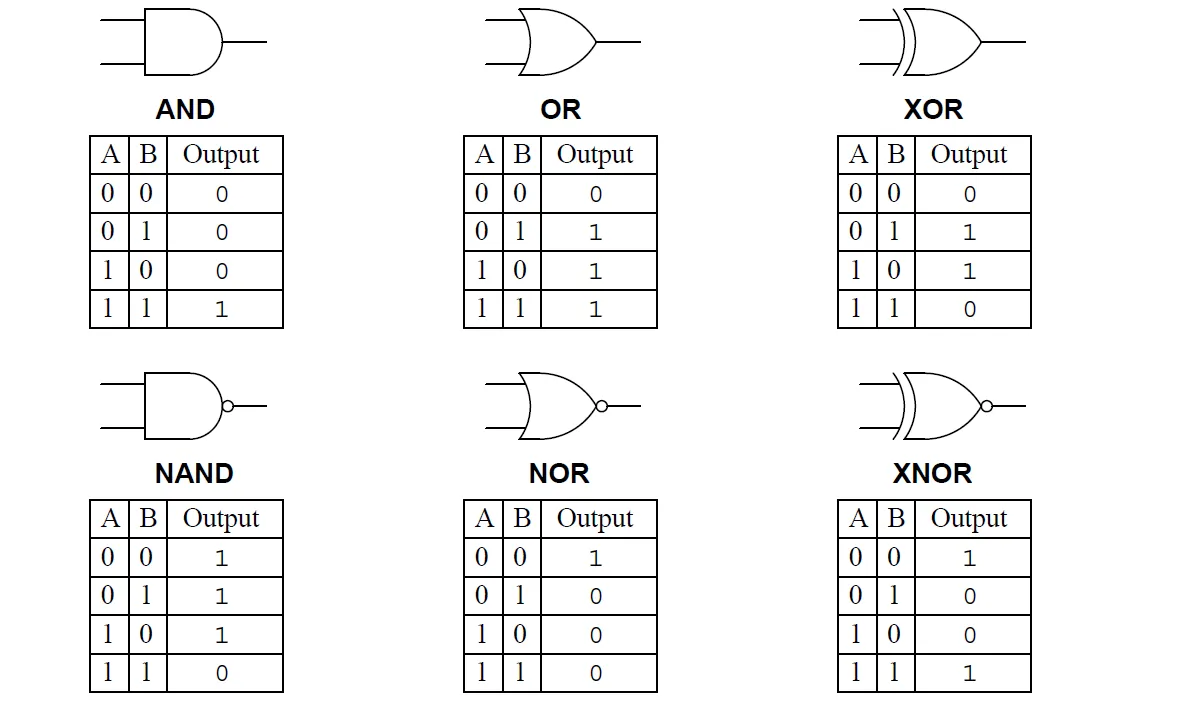
\includegraphics[width=1.0\linewidth]{images/2_le_architetture/logic_gates_truthtables.png}
%		\caption{Le tabelle di verità}
	\end{figure}
	
\end{frame}



\subsection[L'architettura di un computer]{L'architettura di un computer}
\begin{frame}
	\frametitle{L'architettura di un computer}
	
	\begin{block}{L'architettura di un computer}
		L'\textbf{architettura di un computer} comprende tutte le \textbf{scelte progettuali} che vengono fatte durante la creazione di un computer, come ad esempio la scelta dei \textbf{componenti hardware}, la scelta del \textbf{sistema operativo} e il modo in cui tutti questi elementi lavorano insieme per eseguire le istruzioni del software.
	\end{block}
	
	\begin{figure}[!htbp]
		\centering 
		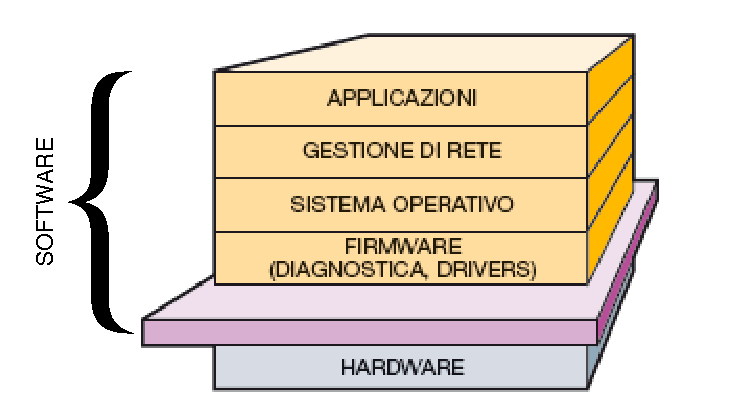
\includegraphics[width=0.6\linewidth]{images/2_le_architetture/hd-sw.pdf}
%			\caption{}
	\end{figure}
	
\end{frame}


\begin{frame}
	\frametitle{L'architettura di un computer}
	
	\begin{block}{L'architettura di un computer}
		In generale, l'architettura di un computer può essere divisa in tre parti principali:
		\begin{itemize}
			\item il processore
			\item la memoria
			\item l'input/output (I/O)
		\end{itemize}
	\end{block}
	
%	\begin{figure}[!htbp]
%		\centering 
%		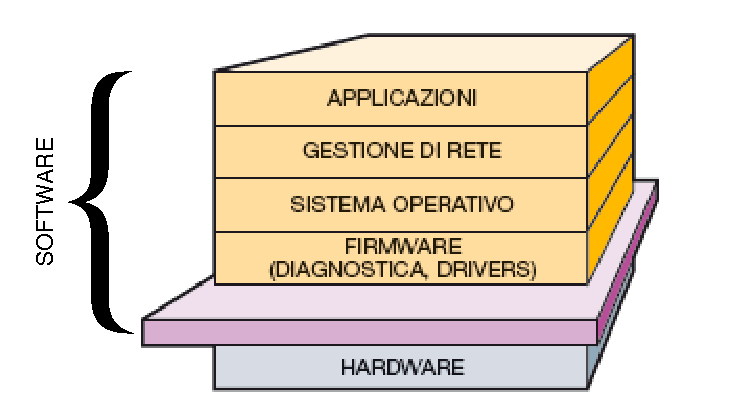
\includegraphics[width=0.6\linewidth]{images/2_le_architetture/hd-sw.pdf}
%%			\caption{}
%	\end{figure}
	
\end{frame}


\begin{frame}
%	\frametitle{L'architettura di un computer}
	
	\begin{block}{Il processore}
		Il \textbf{processore}, noto anche come "microprocessore", è il "cervello" del computer, ed è responsabile dell'esecuzione delle istruzioni contenute nel software.
	\end{block}

	\begin{columns}			
		\column{0.5\linewidth}
		\begin{figure}[!htbp] 
			\centering
			%\advance\leftskip-0.25cm
			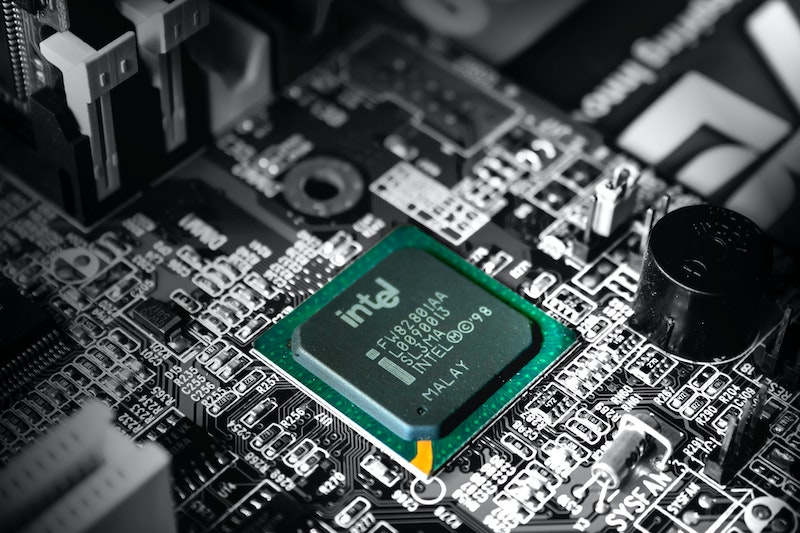
\includegraphics[width=1.0\linewidth]{images/2_le_architetture/intel.jpg}
			\caption{Processore Intel}
			\label{fig:architectures_intel}
		\end{figure}
					
		\column{0.5\linewidth}
		\begin{figure}[!htbp] 
			\centering
			%\advance\leftskip-0.25cm
			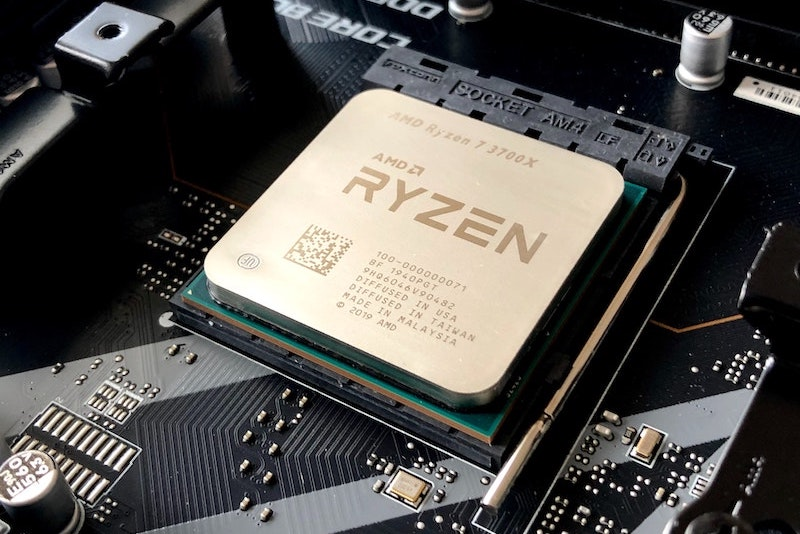
\includegraphics[width=1.0\linewidth]{images/2_le_architetture/ryzen.jpg}
			\caption{Processore AMD Ryzen}
			\label{fig:architectures_ryzen}
		\end{figure}
		
	\end{columns}
	
\end{frame}




\begin{frame}
%	\frametitle{L'architettura di un computer}
	
	\begin{block}{La memoria}
		La \textbf{memoria} è dove vengono temporaneamente archiviati i dati e le istruzioni che vengono utilizzati dal processore. Esistono due tipi principali di memoria: 
		\begin{itemize}
			\item la \textbf{memoria RAM} (Random Access Memory), che viene utilizzata per archiviare i dati che il processore sta attualmente lavorando
			\item la \textbf{memoria di massa}, come il disco rigido o il solid state drive, che viene utilizzata per archiviare i dati a lungo termine.
		\end{itemize}
	\end{block}
	
	\begin{columns}			
		\column{0.5\linewidth}
		\begin{figure}[!htbp]
			\centering
			%\advance\leftskip-0.25cm
			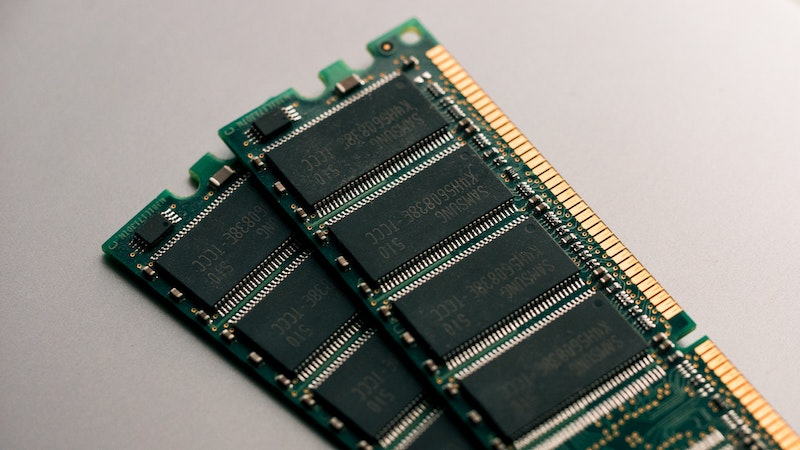
\includegraphics[width=0.82\linewidth]{images/2_le_architetture/memory_ram.jpg}
			\caption{Due memorie RAM}
			\label{fig:architectures_memory_ram}
		\end{figure}
					
		\column{0.5\linewidth}
		\begin{figure}[!htbp] 
			\centering
			%\advance\leftskip-0.25cm
			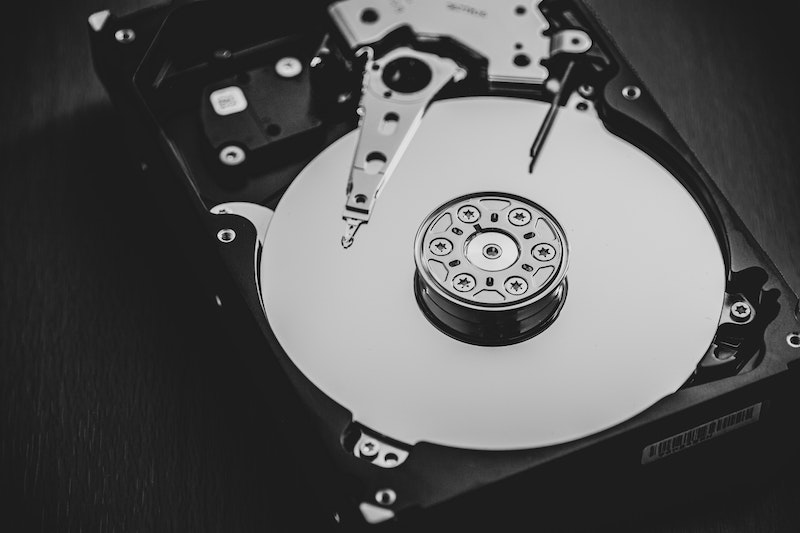
\includegraphics[width=0.7\linewidth]{images/2_le_architetture/memory_hdd.jpg}
			\caption{L'interno di un Hard Disk}
			\label{fig:architectures_memory_hdd}
		\end{figure}
		
	\end{columns}
	
\end{frame}


\begin{frame}
%	\frametitle{L'architettura di un computer}
	
	\begin{block}{L'input/output (I/O)} 
		L'\textbf{input/output} (I/O) gestisce il flusso di dati tra il computer e l'esterno, attraverso dispositivi come il monitor, la tastiera e il mouse.
	\end{block}
	
	\begin{figure}[!htbp] 
		\centering
		%\advance\leftskip-0.25cm
		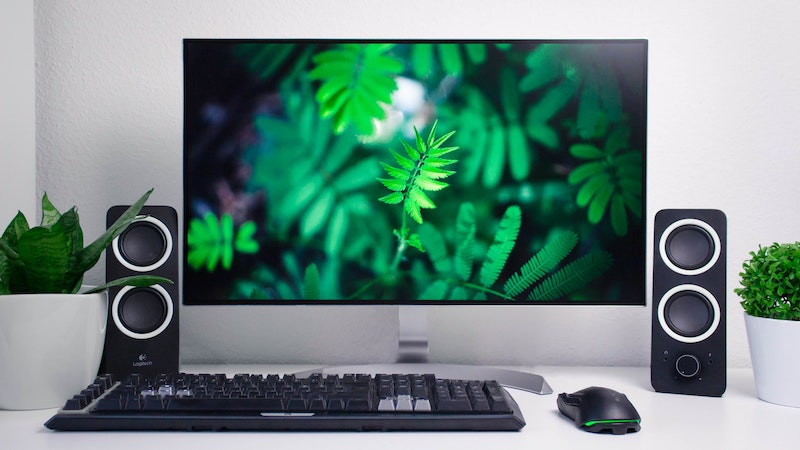
\includegraphics[width=0.8\linewidth]{images/2_le_architetture/io.jpg}
		\caption{Monitor, tastiera, mouse e casse}
		\label{fig:architectures_io}
	\end{figure}
	 
\end{frame}


\begin{frame}
%	\frametitle{L'architettura di un computer}
	
	\begin{block}{Altre componenti}
		Altre componenti comuni di un computer possono includere schede di espansione, che forniscono ulteriori funzionalità al computer, come ad esempio la possibilità di collegare dispositivi esterni o di aggiungere ulteriori porte di I/O.
	\end{block}
	
%	\begin{figure}[!htbp]
%		\centering 
%		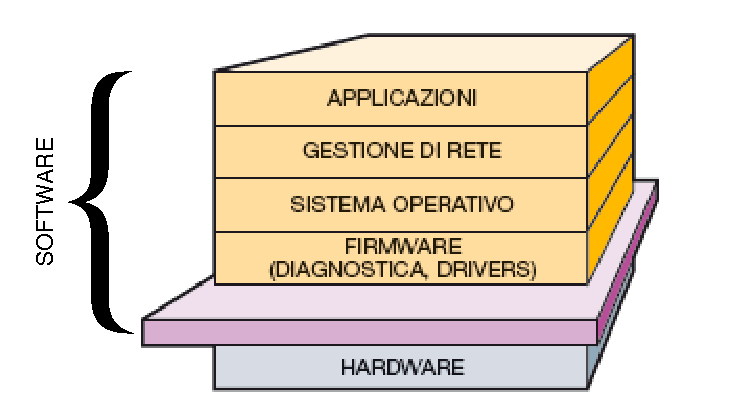
\includegraphics[width=0.6\linewidth]{images/2_le_architetture/hd-sw.pdf}
%%			\caption{}
%	\end{figure}
	
\end{frame}



